% MetroMitra -- Architecture Document (no-backend / Idea Junction edition)
% LaTeX source. Compile with pdflatex, xelatex, or tectonic.
% Reflects the v2 architecture: client-side Zustand + localStorage,
% demo auth, static station reference data, and the Idea Junction feature.

\documentclass[a4paper,11pt]{article}

\usepackage[T1]{fontenc}
\usepackage[utf8]{inputenc}
\usepackage[margin=2.5cm]{geometry}
\usepackage{lmodern}
\usepackage{microtype}
\usepackage{amsmath}
\usepackage{xcolor}
\usepackage{tikz}
\usetikzlibrary{positioning, arrows.meta, shapes.geometric, fit, calc, backgrounds}
\usepackage{listings}
\usepackage{booktabs}
\usepackage{enumitem}
\usepackage{caption}
\usepackage{titlesec}

% --- Brand palette ----------------------------------------------------------
\definecolor{terracotta}{HTML}{C2410C}
\definecolor{terracottasoft}{HTML}{F97316}
\definecolor{terracottatint}{HTML}{FED7AA}
\definecolor{canvas}{HTML}{FAF7F2}
\definecolor{ink}{HTML}{1F1B16}
\definecolor{slate}{HTML}{475569}

% Metro line palette (used in the Idea Junction concept diagram)
\definecolor{metroblue}{HTML}{2563EB}
\definecolor{metroyellow}{HTML}{EAB308}
\definecolor{metrogreen}{HTML}{16A34A}
\definecolor{metropurple}{HTML}{9333EA}
\definecolor{metrored}{HTML}{DC2626}
\definecolor{metroaqua}{HTML}{0891B2}

% --- Hyperref (load late, before bookmark) ---------------------------------
\usepackage[hidelinks]{hyperref}
\hypersetup{
  colorlinks=true,
  linkcolor=terracotta,
  urlcolor=terracotta,
  citecolor=terracotta,
  pdftitle={MetroMitra Architecture (no-backend / Idea Junction edition)},
  pdfauthor={MetroMitra Engineering},
  pdfsubject={Architecture document for MetroMitra v2},
  pdfkeywords={MetroMitra, Next.js, Zustand, localStorage, Idea Junction, TikZ}
}
\usepackage{bookmark}

% --- Section formatting -----------------------------------------------------
\titleformat{\section}{\color{terracotta}\Large\bfseries\sffamily}{\thesection}{0.8em}{}
\titleformat{\subsection}{\color{terracotta}\large\bfseries\sffamily}{\thesubsection}{0.6em}{}
\titleformat{\subsubsection}{\color{ink}\normalsize\bfseries\sffamily}{\thesubsubsection}{0.5em}{}
\titlespacing*{\section}{0pt}{14pt}{6pt}
\titlespacing*{\subsection}{0pt}{10pt}{4pt}

% --- Caption formatting -----------------------------------------------------
\captionsetup{font=small, labelfont={bf,color=terracotta}, format=plain, justification=raggedright, singlelinecheck=false, skip=4pt}

% --- Listings (TypeScript) --------------------------------------------------
\lstdefinelanguage{TypeScript}{
  morekeywords={const, let, var, function, return, async, await, import, from, export, default, type, interface, extends, implements, new, class, public, private, if, else, for, while, try, catch, throw, true, false, null, undefined, as, in, of, switch, case, break, continue, string, number, boolean, Promise, Array, Record, unknown, void, never, Partial, Pick, Omit},
  sensitive=true,
  morecomment=[l]{//},
  morecomment=[s]{/*}{*/},
  morestring=[b]',
  morestring=[b]",
  morestring=[b]`,
}

\lstset{
  language=TypeScript,
  basicstyle=\ttfamily\footnotesize,
  keywordstyle=\color{terracotta}\bfseries,
  commentstyle=\color{slate!75}\itshape,
  stringstyle=\color{teal!70!black},
  identifierstyle=\color{ink},
  backgroundcolor=\color{canvas},
  frame=leftline,
  rulecolor=\color{terracotta},
  framerule=1.2pt,
  framesep=8pt,
  xleftmargin=10pt,
  xrightmargin=2pt,
  showstringspaces=false,
  breaklines=true,
  breakatwhitespace=true,
  tabsize=2,
  aboveskip=10pt,
  belowskip=8pt,
}

\renewcommand{\emergencystretch}{3em}

% --- TikZ shared styles -----------------------------------------------------
\tikzset{
  block/.style={draw=terracotta, line width=0.9pt, rounded corners=2pt, fill=canvas, align=center, font=\small\sffamily, minimum height=8mm, inner sep=6pt},
  box/.style={draw=slate!60, line width=0.6pt, rounded corners=2pt, fill=white, align=center, font=\small\sffamily, minimum height=8mm, inner sep=6pt},
  store/.style={draw=terracotta, line width=1pt, fill=terracottatint!50, align=center, font=\small\sffamily, minimum height=10mm, inner sep=8pt},
  static/.style={draw=metrogreen, line width=0.9pt, fill=metrogreen!10, align=center, font=\small\sffamily, minimum height=8mm, inner sep=6pt},
  entity/.style={draw=slate!70, line width=0.7pt, fill=canvas, align=center, font=\footnotesize\sffamily, minimum height=7mm, inner sep=4pt},
  staticentity/.style={draw=metrogreen!80, line width=0.7pt, fill=metrogreen!8, align=center, font=\footnotesize\sffamily, minimum height=7mm, inner sep=4pt},
  demoentity/.style={draw=terracotta!80, line width=0.7pt, fill=terracotta!8, align=center, font=\footnotesize\sffamily, minimum height=7mm, inner sep=4pt},
  arrow/.style={-{Stealth[length=2.4mm]}, line width=0.7pt, draw=slate!80},
  flow/.style={-{Stealth[length=2.4mm]}, line width=0.9pt, draw=terracotta},
  dashedarrow/.style={-{Stealth[length=2.4mm]}, line width=0.6pt, draw=slate!70, dashed},
}

% Suppress the duplicate page-anchor warning around the title page.
\hypersetup{pageanchor=false}

\begin{document}

% ============================================================================
%  TITLE PAGE
% ============================================================================

\begin{titlepage}
\centering
\vspace*{1.5cm}

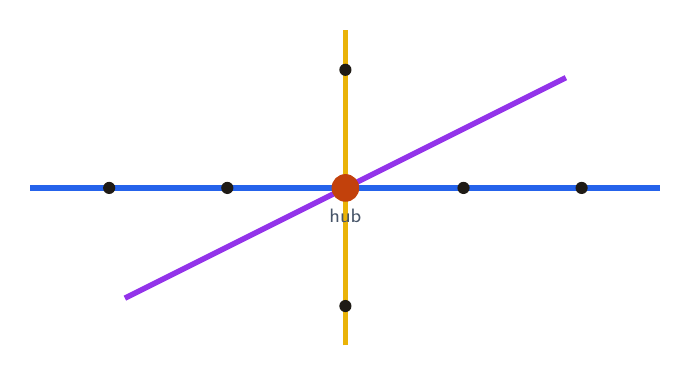
\begin{tikzpicture}[remember picture]
  % Small metro-map motif: three lines crossing at a hub, with station dots.
  \draw[metroblue, line width=2pt] (-4,0) -- (4,0);
  \draw[metroyellow, line width=2pt] (0,-2) -- (0,2);
  \draw[metropurple, line width=2pt] (-2.8,-1.4) -- (2.8,1.4);
  \foreach \x in {-3,-1.5,0,1.5,3} \fill[ink] (\x,0) circle (2.2pt);
  \foreach \y in {-1.5,0,1.5} \fill[ink] (0,\y) circle (2.2pt);
  \fill[terracotta] (0,0) circle (5pt);
  \node[font=\scriptsize\sffamily, color=slate] at (0.0,-0.35) {hub};
\end{tikzpicture}

\vspace{1.2cm}
{\color{terracotta}\sffamily\Huge\bfseries MetroMitra}\\[4pt]
{\color{slate}\sffamily\Large Architecture Document}\\[2pt]
{\color{slate}\sffamily\normalsize v2 -- No-backend edition, with Idea Junction}

\vspace{2.2cm}
\begin{minipage}{0.82\textwidth}
\centering\small\color{slate}
A client-side Next.js application for Indian metro commuters.
All data lives in the browser via Zustand with \texttt{localStorage} persistence.
Authentication is a demo context (not for production). The "travel buddy finder"
feature has been retired and replaced by \emph{Idea Junction}, a station-anchored
entrepreneurial ideas and discussion board. This document describes the
architecture, the local data model, the auth flow, the feature set, the
deployment topology, and the honest limitations of the no-backend approach.
\end{minipage}

\vfill
{\color{slate}\sffamily\small MetroMitra Engineering \quad\textbullet\quad \today}
\end{titlepage}

\hypersetup{pageanchor=true}

\begin{abstract}
\noindent
MetroMitra is a hyperlocal community web app for Indian metro commuters, covering
six cities and thirty-nine real stations. The version described here is built
without a backend, without a database, and without an API layer. The browser is
the only runtime: a Next.js client bundle holds a Zustand store, persistence is
\texttt{localStorage}, and station reference data ships as a static TypeScript
module. Authentication is a deliberately thin client-side context with a demo
hash, intended for functionality exploration rather than production use. The
former travel-buddy-finder feature has been removed and replaced by Idea
Junction, a station-anchored board for entrepreneurial ideas, validation
questions, and cofounder search. This document records the system architecture,
the local data model, the auth flow, each feature and its store interactions,
the deployment topology on Vercel via GitHub Actions, the security and privacy
posture (with an honest accounting of what is and is not safe), accessibility
and performance notes, and the migration path to a real backend if the product
ever outgrows the demo.
\end{abstract}

\vspace{0.6cm}
\tableofcontents
\newpage

% ============================================================================
%  1. INTRODUCTION
% ============================================================================

\section{Introduction}

MetroMitra is a community application for people who ride the metro in Indian
cities. It treats the metro not as a transport utility but as a social graph:
riders who share a station also share a routine, a neighbourhood, and a chunk of
their day. The product surfaces that overlap to support community posts,
last-mile carpools, lost-and-found, a station-scoped marketplace, and the
flagship feature of this release, Idea Junction.

The original design of MetroMitra used a conventional stack: Next.js with
Prisma, SQLite, NextAuth, and a set of REST route handlers. That stack is gone.
The version documented here has no backend, no database, and no API. Everything
the user creates lives in their own browser. The reasoning is straightforward
and worth stating plainly. The point of this release is to explore
functionality and product fit, not to operate a service. Removing the server
removes a long list of incidental complexity: schema migrations, connection
pooling, session storage, password reset flows, rate limiting, hosting for the
database, and the entire class of bugs where the client and server disagree
about the shape of a record. What remains is an application that runs after
\texttt{npm install} and \texttt{npm run dev}, with no provisioning step at
all.

The second change in this release is a feature pivot. The earlier travel buddy
finder, which paired commuters who wanted company for a metro leg, has been
retired. In its place is Idea Junction: a station-anchored board where
commuters post entrepreneurial ideas, side-project thoughts, startup concepts,
or validation questions, and look for cofounders, collaborators, feedback, or
discussion among people who ride the same metro line. The insight is that metro
commuters are disproportionately young professionals, students, and aspiring
founders, and that matching them by station ties serendipity to physical
proximity and shared routine. Commute time becomes a venue for entrepreneurial
conversation. Section~\ref{sec:idea-junction} treats the feature in detail.

The rest of this document is organised as a conventional architecture review.
We cover the system, the stack, the local data model, the demo auth flow, the
features, the frontend architecture, deployment, security, accessibility and
performance, limitations, and the conclusion. Throughout, the prose is honest
about what is demo-grade. A production version of MetroMitra would need a real
backend; we sketch that migration path in section~\ref{sec:limitations}.

% ============================================================================
%  2. SYSTEM OVERVIEW
% ============================================================================

\section{System overview}

The system is a single-page Next.js application that runs entirely in the
browser. There is no application server, no API gateway, no database, and no
background worker. The Next.js build produces a static and edge-rendered
bundle served by Vercel; the only server-side code is the rendering of public
pages (the landing page, the station directory, the sitemap, and the robots
file) and those do not touch any data source beyond the static station module.
Figure~\ref{fig:system} shows the topology.

\begin{figure}[ht]
\centering
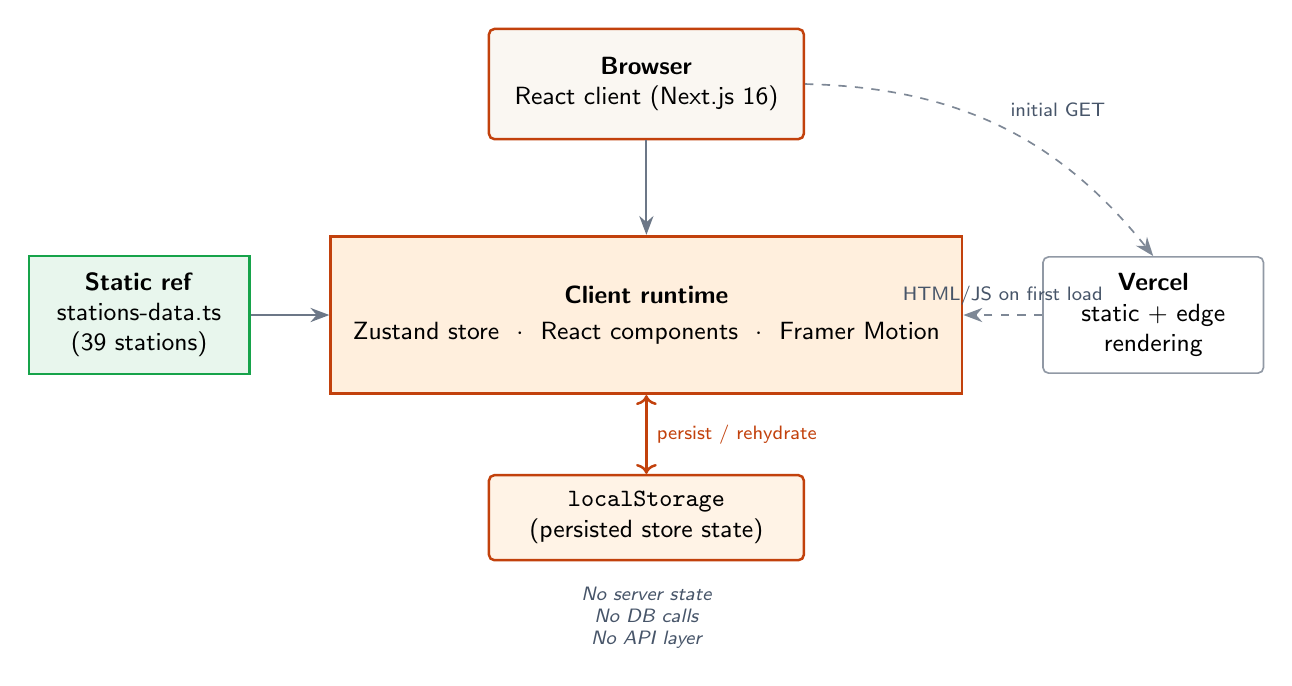
\begin{tikzpicture}[node distance=10mm and 10mm]
  % Browser client
  \node[block, minimum width=40mm, minimum height=14mm] (browser)
    {\textbf{Browser}\\React client (Next.js 16)};
  % Inside the browser: a container
  \node[store, below=12mm of browser, minimum width=68mm, minimum height=20mm,
        fill=terracottatint!40, draw=terracotta, line width=1pt] (client)
    {\textbf{Client runtime}\\[2pt]
     Zustand store\ \ $\cdot$\ \ React components\ \ $\cdot$\ \ Framer Motion};
  % LocalStorage
  \node[block, below=10mm of client, minimum width=40mm, minimum height=10mm,
        fill=terracottatint!30] (ls)
    {\texttt{localStorage}\\(persisted store state)};
  % Static station data
  \node[static, left=10mm of client, minimum width=28mm, minimum height=14mm] (stations)
    {\textbf{Static ref}\\stations-data.ts\\(39 stations)};
  % Edge / Vercel hosting
  \node[box, right=10mm of client, minimum width=28mm, minimum height=14mm] (vercel)
    {\textbf{Vercel}\\static + edge\\rendering};

  % Edges
  \draw[arrow] (browser) -- (client.north);
  \draw[flow, <->] (client) -- node[right, font=\scriptsize\sffamily, color=terracotta] {persist / rehydrate} (ls);
  \draw[arrow] (stations) -- (client);
  \draw[dashedarrow] (vercel) -- node[above, font=\scriptsize\sffamily, color=slate] {HTML/JS on first load} (client);
  \draw[dashedarrow] (browser.east) to[bend left=25] node[above right, font=\scriptsize\sffamily, color=slate] {initial GET} (vercel.north);

  % "No" annotations
  \node[font=\scriptsize\sffamily\itshape, color=slate, below=2mm of ls, align=center]
    {No server state\\No DB calls\\No API layer};
\end{tikzpicture}
\caption{System architecture. The browser is the only runtime. The Zustand
store is the single source of truth for user-generated data;
\texttt{localStorage} provides persistence across page reloads. Station
reference data is a static TypeScript module imported into the bundle. Vercel
serves the static and edge-rendered output of \texttt{next build}.}
\label{fig:system}
\end{figure}

The design suits the current stage of the product. A functionality-exploration
demo lives or dies on whether a reviewer can open it, create a post, join a
carpool, and post an idea in under a minute. A backend in the loop would mean
provisioning a database, configuring connection strings, running migrations,
and reasoning about cold starts. None of that helps a reviewer understand
whether the product concept holds. The local-memory approach also has a
pedagogical virtue: every action is fully traceable in the browser devtools.
The store, the persisted state, and the rendered output are all in one place.

The cost is real, and we discuss it throughout. Data does not leave the
browser. Two users on two devices cannot see each other's posts. State is
ephemeral in the sense that it is per-browser, although it survives reloads.
For a demo this is acceptable. For a product with real users it would not be,
and section~\ref{sec:limitations} sketches the migration.

% ============================================================================
%  3. TECHNOLOGY STACK AND RATIONALE
% ============================================================================

\section{Technology stack and rationale}

The stack is small and intentionally conventional. Each choice is justified by
the Ponytail principle: the simplest correct implementation for the current
stage of the product, with the option to grow if needed.

\textbf{Next.js 16} is the application framework. It gives us file-based
routing, the App Router, server components for the public pages that benefit
from static rendering (landing, station directory, sitemap), and client
components for the interactive app. We use Next.js not for its server
capabilities in this release but because the routing model, the build
pipeline, and the Vercel deployment story are familiar and stable. Choosing a
lighter bundler would buy very little and cost us a generation of tooling.

\textbf{TypeScript} is non-negotiable. The local store has a richer shape
than the average React state because it carries users, posts, carpools, ideas,
marketplace listings, contact requests, and ratings in one tree. TypeScript
makes that shape navigable and catches the class of bugs where a feature
mutates a field that another feature reads. Strict mode is on.

\textbf{Tailwind CSS 4} handles styling. The utility-class approach keeps the
component surface small and the design tokens consistent. We define the brand
palette as Tailwind tokens, so the terracotta accent and the metro-line
colours used in Idea Junction badges are the same values that appear in the
TikZ diagrams in this document.

\textbf{shadcn/ui} provides a small set of accessible primitives (dialog,
sheet, button, input, select, card, toast). We use shadcn rather than a
packaged component library because the components are copied into the
repository and owned by us; there is no version skew, no hidden behaviour, and
no dependency on a library's release cadence.

\textbf{Zustand with the persist middleware} is the state container. Zustand's
model is a single store with subscriptions and selectors, and the persist
middleware writes every state change to \texttt{localStorage} under a
configurable key. We picked Zustand over Redux because the boilerplate is much
lower and the mental model is a plain object with methods, not a reducer
graph. We picked it over React Context alone because Context re-renders every
consumer on any change, which gets expensive when the store carries a full
social feed.

\textbf{Framer Motion} handles animation, used at level 1 only: small
transitions on hover, on dialog open, on tab change. Nothing decorates the
page for its own sake.

\subsection{What we rejected, and why}

The earlier MetroMitra stack was Prisma with SQLite, NextAuth for sessions,
and a set of REST route handlers under \texttt{src/app/api/*}. We removed all
of it. The reasons are practical, not ideological.

Prisma and SQLite were the most expensive part of the demo to maintain. They
required a schema file, a generated client, a migration step, a seeded
database, and a writable filesystem on the host. On Vercel the filesystem is
ephemeral, so the database reset on every cold start unless we provisioned an
external store. For a functionality demo we did not need cross-user data
sharing, so the entire dependency added setup cost without product value.

NextAuth was the second expense. It required an authentication secret, a
session strategy, a credentials provider, and careful handling of the
\texttt{/api/auth/*} callbacks. The demo auth context described in
section~\ref{sec:auth} does the same job for a demo in roughly fifty lines of
TypeScript, with no secrets and no server round-trip.

The REST route handlers were the third. Each feature had a POST, a GET, a
PATCH, and usually a nested resource (for example, joining a carpool). That
is roughly thirty handlers, each with input validation, error handling, and
its own small surface area for bugs. In the new architecture every feature is
a Zustand action plus a React component. The action mutates the local store,
the persist middleware writes to \texttt{localStorage}, and the selector
re-renders the view. There is no network call to fail.

% ============================================================================
%  4. LOCAL DATA MODEL
% ============================================================================

\section{Local data model}

The store is a single Zustand tree. On creation it is hydrated from
\texttt{localStorage} if a previous session wrote one; otherwise it is seeded
with a small set of demo content (a couple of demo users, a few starter
posts, an example carpool, and one example idea) so that a fresh reviewer sees
a populated app rather than an empty shell. The static station data is
imported from \texttt{src/lib/stations-data.ts} and is not part of the
persisted store; it is reference data, immutable, and ships in the bundle.

Figure~\ref{fig:entities} shows the conceptual entity model. Solid
terracotta-bordered entities are persisted in the store. The green-bordered
Station is static reference data. The two demo entities (User and
ContactRequest) are tinted to remind the reader that they are demo-grade.

\begin{figure}[ht]
\centering
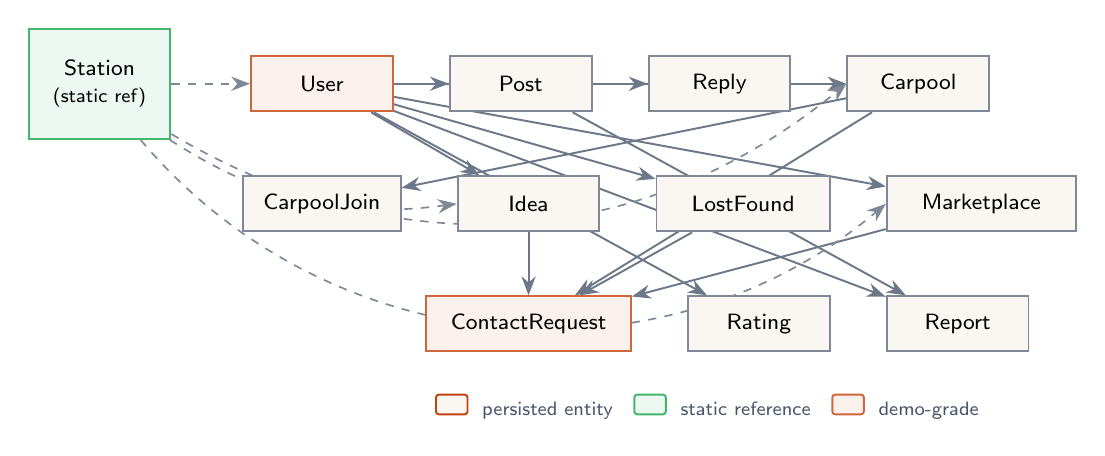
\begin{tikzpicture}[node distance=5mm and 7mm]
  % Station reference (left column)
  \node[staticentity, minimum width=18mm, minimum height=14mm] (station)
    {Station\\\scriptsize(static ref)};

  % Row 1: User, Post, Reply, Carpool
  \node[demoentity, right=10mm of station, minimum width=18mm] (user) {User};
  \node[entity, right=of user, minimum width=18mm] (post) {Post};
  \node[entity, right=of post, minimum width=18mm] (reply) {Reply};
  \node[entity, right=of reply, minimum width=18mm] (carpool) {Carpool};

  % Row 2 (below row 1): CarpoolJoin, Idea, LostFound, Marketplace
  \node[entity, below=8mm of user, minimum width=20mm] (cjoin) {CarpoolJoin};
  \node[entity, right=of cjoin, minimum width=18mm] (idea) {Idea};
  \node[entity, right=of idea, minimum width=22mm] (lostfound) {LostFound};
  \node[entity, right=of lostfound, minimum width=24mm] (market) {Marketplace};

  % Row 3 (below row 2): ContactRequest, Rating, Report
  \node[demoentity, below=8mm of idea, minimum width=26mm] (contact) {ContactRequest};
  \node[entity, right=of contact, minimum width=18mm] (rating) {Rating};
  \node[entity, right=of rating, minimum width=18mm] (report) {Report};

  % Edges (drawn behind via backgrounds layer)
  \begin{pgfonlayer}{background}
    \draw[arrow] (user) -- (post);
    \draw[arrow] (post) -- (reply);
    \draw[arrow] (user) -- (carpool);
    \draw[arrow] (carpool) -- (cjoin);
    \draw[arrow] (user) -- (idea);
    \draw[arrow] (user) -- (lostfound);
    \draw[arrow] (user) -- (market);
    \draw[arrow] (idea) -- (contact);
    \draw[arrow] (carpool) -- (contact);
    \draw[arrow] (lostfound) -- (contact);
    \draw[arrow] (market) -- (contact);
    \draw[arrow] (user) -- (rating);
    \draw[arrow] (user) -- (report);
    \draw[arrow] (post) -- (report);

    % Station is referenced by nearly everything; show a few representative edges.
    \draw[dashedarrow] (station) -- (user);
    \draw[dashedarrow] (station) to[bend right=20] (idea.west);
    \draw[dashedarrow] (station) to[bend right=35] (carpool.west);
    \draw[dashedarrow] (station) to[bend right=45] (market.west);
  \end{pgfonlayer}

  % Legend (below the diagram)
  \node[font=\scriptsize\sffamily, color=slate, align=left, anchor=north west]
    at ([yshift=-4mm]contact.south west) {
    \tikz\draw[draw=terracotta, fill=canvas, line width=0.7pt, rounded corners=1pt] (0,0) rectangle (4mm,2.5mm);~ persisted entity\quad
    \tikz\draw[draw=metrogreen!80, fill=metrogreen!8, line width=0.7pt, rounded corners=1pt] (0,0) rectangle (4mm,2.5mm);~ static reference\quad
    \tikz\draw[draw=terracotta!80, fill=terracotta!8, line width=0.7pt, rounded corners=1pt] (0,0) rectangle (4mm,2.5mm);~ demo-grade
  };
\end{tikzpicture}
\caption{Conceptual entity model of the local store. Solid terracotta-bordered
entities are persisted to \texttt{localStorage} by the Zustand persist
middleware. Station (green) is static reference data, imported into the bundle
and never mutated. User and ContactRequest are tinted to flag that they are
demo-grade. Station is referenced by every user-generated entity; we draw a
representative subset of those edges.}
\label{fig:entities}
\end{figure}

\subsection{Store shape and persistence}

The store is one object with a fixed set of slices: \texttt{users},
\texttt{currentUserId}, \texttt{posts}, \texttt{replies}, \texttt{carpools},
\texttt{carpoolJoins}, \texttt{ideas}, \texttt{lostFound}, \texttt{marketplace},
\texttt{contactRequests}, \texttt{ratings}, and \texttt{reports}. Each slice is
an array of records, with the exception of \texttt{currentUserId}, which is a
string or \texttt{null}. The persist middleware serialises the entire object to
\texttt{localStorage} under the key \texttt{metromitra-store} on every state
change. On application boot, Zustand rehydrates from that key synchronously
before the first render, so the UI never flashes an empty state on a return
visit.

\subsection{Static station reference data}

The file \texttt{src/lib/stations-data.ts} exports an array of
\texttt{StationSeed} records. Each record carries a short code (for example
\texttt{MGR} for MG Road, Bengaluru), the station name, the city, a
comma-separated list of metro lines it serves, the matching list of line
colours, and an optional exit count. The file also exports the list of cities
and a mapping from line colour name to its hex value, so the UI can render
metro-line badges without an indirection. The dataset is thirty-nine stations
across six cities: Delhi, Mumbai, Bengaluru, Hyderabad, Chennai, and Kolkata.
These are reference data, not user input; the only mutations on the station
array happen in tests, never in the running app.

\subsection{Demo seeding on first load}

On the very first load, when \texttt{localStorage} has no
\texttt{metromitra-store} key, the store initialises with a small set of demo
content so the app is explorable. This includes two or three demo users (with
lightly hashed passwords known to the README), a handful of community posts
spread across stations in different cities, an example carpool for an evening
last-mile leg, one or two lost-and-found entries, a marketplace listing, and
one example Idea Junction post in each of the \texttt{idea},
\texttt{cofounder}, and \texttt{feedback} categories. The seed runs exactly
once per browser; subsequent loads hydrate from \texttt{localStorage} and
preserve whatever the user has added.

% ============================================================================
%  5. CLIENT-SIDE AUTHENTICATION
% ============================================================================

\section{Client-side authentication}
\label{sec:auth}

Authentication is a thin React context backed by the same Zustand store. The
flow has three operations: register, login, and logout. Figure~\ref{fig:auth}
shows the three paths.

\begin{figure}[ht]
\centering
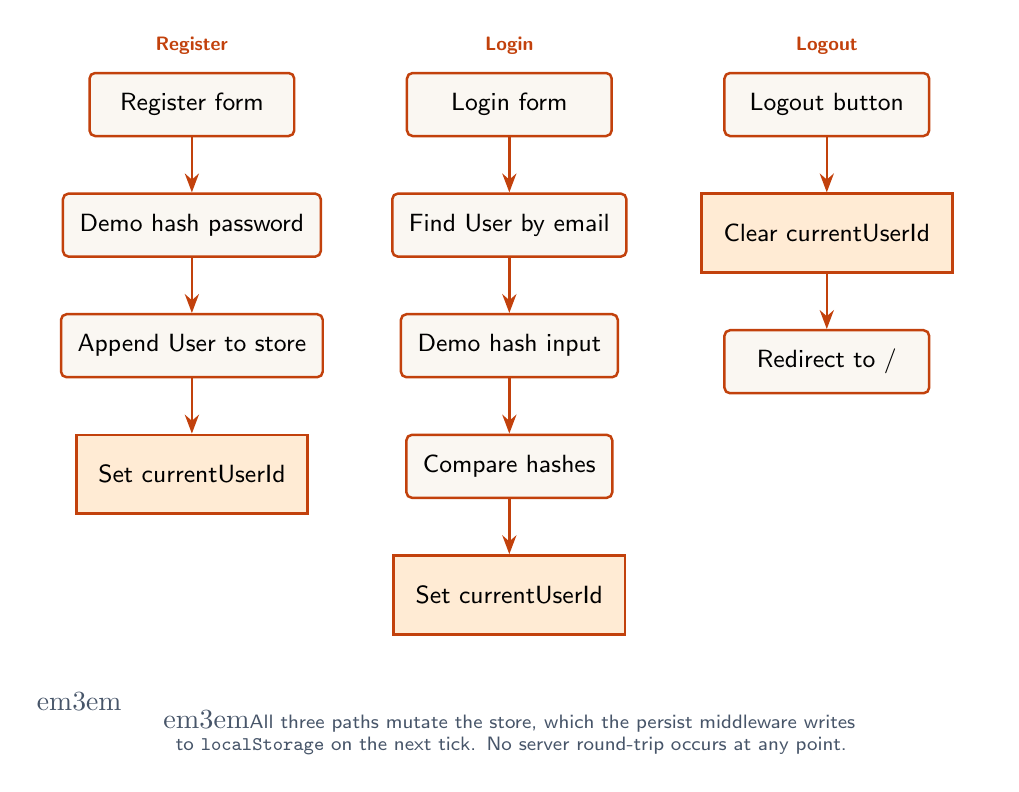
\begin{tikzpicture}[node distance=7mm and 8mm]
  % Three columns: Register / Login / Logout
  % Register column
  \node[block, minimum width=26mm] (r1) {Register form};
  \node[block, below=of r1, minimum width=26mm] (r2) {Demo hash password};
  \node[block, below=of r2, minimum width=26mm] (r3) {Append User to store};
  \node[store, below=of r3, minimum width=26mm] (r4) {Set currentUserId};
  \draw[flow] (r1) -- (r2);
  \draw[flow] (r2) -- (r3);
  \draw[flow] (r3) -- (r4);
  \node[font=\scriptsize\sffamily, color=terracotta, above=1mm of r1] {\textbf{Register}};

  % Login column
  \node[block, right=14mm of r1, minimum width=26mm] (l1) {Login form};
  \node[block, below=of l1, minimum width=26mm] (l2) {Find User by email};
  \node[block, below=of l2, minimum width=26mm] (l3) {Demo hash input};
  \node[block, below=of l3, minimum width=26mm] (l4) {Compare hashes};
  \node[store, below=of l4, minimum width=26mm] (l5) {Set currentUserId};
  \draw[flow] (l1) -- (l2);
  \draw[flow] (l2) -- (l3);
  \draw[flow] (l3) -- (l4);
  \draw[flow] (l4) -- (l5);
  \node[font=\scriptsize\sffamily, color=terracotta, above=1mm of l1] {\textbf{Login}};

  % Logout column
  \node[block, right=14mm of l1, minimum width=26mm] (o1) {Logout button};
  \node[store, below=of o1, minimum width=26mm] (o2) {Clear currentUserId};
  \node[block, below=of o2, minimum width=26mm] (o3) {Redirect to /};
  \draw[flow] (o1) -- (o2);
  \draw[flow] (o2) -- (o3);
  \node[font=\scriptsize\sffamily, color=terracotta, above=1mm of o1] {\textbf{Logout}};

  % Persistence annotation, centred under all three columns
  \node[font=\scriptsize\sffamily, color=slate, below=6mm of l5, align=center, text width=120mm]
    (note) {All three paths mutate the store, which the persist middleware writes to
            \texttt{localStorage} on the next tick. No server round-trip occurs at any point.};
\end{tikzpicture}
\caption{Client-side authentication flow. Register hashes the password with a
demo hash, appends a User record to the store, and sets the current user.
Login finds the user by email, hashes the input, and compares. Logout clears
the current user. None of these operations touch the network.}
\label{fig:auth}
\end{figure}

The demo hash is a deliberately weak one-way function, not a cryptographic
password hash. We use it so that passwords are not stored in plaintext in
\texttt{localStorage}, which would make them visible to anyone with devtools
access. A reviewer who opens devtools sees a hash, not a password. That is the
full extent of the protection. The hash is not salted per user, is not
resistant to brute force, and would be considered broken in any production
context. We accept it because the alternative in a no-backend demo is to store
passwords in plaintext, which is worse, or to ship a full client-side crypto
stack, which adds complexity the demo does not need.

The session is the \texttt{currentUserId} field in the store, persisted to
\texttt{localStorage}. A page reload restores the session. A logout clears it.
There is no token, no cookie, no expiry, and no server to validate against.
The implication is that anyone with access to the browser can read the store,
modify it, and impersonate any user. For a demo running on a reviewer's own
machine this is fine. For a real product it would be a security incident
waiting to happen, and section~\ref{sec:security} is explicit about what a
production version would need.

% ============================================================================
%  6. FEATURE ARCHITECTURE
% ============================================================================

\section{Feature architecture}

Each feature in MetroMitra follows the same pattern: a slice in the Zustand
store, a set of actions on that slice, a React component that calls the
actions and subscribes to selectors, and a route under \texttt{src/app}. There
is no feature-specific network code because there is no network. The
persistence cycle is the same for every feature and is shown in
figure~\ref{fig:flow}.

\begin{figure}[ht]
\centering
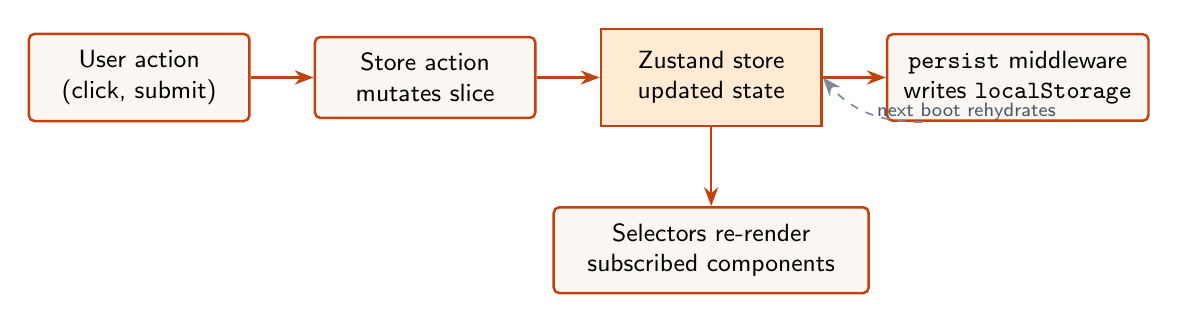
\begin{tikzpicture}[node distance=10mm and 8mm]
  \node[block, minimum width=28mm] (user) {User action\\(click, submit)};
  \node[block, right=of user, minimum width=28mm] (action) {Store action\\mutates slice};
  \node[store, right=of action, minimum width=28mm] (store) {Zustand store\\updated state};
  \node[block, right=of store, minimum width=30mm] (persist) {\texttt{persist} middleware\\writes \texttt{localStorage}};
  \node[block, below=10mm of store, minimum width=40mm] (render) {Selectors re-render\\subscribed components};

  \draw[flow] (user) -- (action);
  \draw[flow] (action) -- (store);
  \draw[flow] (store) -- (persist);
  \draw[flow] (store) -- (render);
  \draw[dashedarrow] (persist) to[bend left=25] node[right, font=\scriptsize\sffamily, color=slate] {next boot rehydrates} (store.east);
\end{tikzpicture}
\caption{The Zustand persist cycle. A user action calls a store action, which
mutates a slice. The persist middleware writes the new state to
\texttt{localStorage}. Subscribed selectors re-render the affected components.
On the next page load, the store rehydrates from \texttt{localStorage} before
first paint.}
\label{fig:flow}
\end{figure}

\textbf{Community feed.} The feed lists posts anchored to a station or city.
A user composes a post with optional station scope; the action appends a
\texttt{Post} record to \texttt{posts} with the author's id and a timestamp.
Replies are nested under a post by id. The feed selector sorts posts
reverse-chronologically and groups replies by parent. There is no pagination
in the demo because the dataset is small; if the dataset grew we would
virtualise the list rather than paginate, since the data is local and
pagination is purely a rendering concern.

\textbf{Last-mile carpool.} A carpool is a ride offer from a station to a
nearby destination, with a time, a seat count, and a status. Other users can
request to join; a \texttt{CarpoolJoin} record is created with status
\texttt{pending}. The driver accepts or declines from their dashboard. The
carpool slice exposes selectors for open carpools at a station, carpools the
current user has offered, and carpools the current user has requested to
join.

\textbf{Idea Junction.} Treated in its own section (section~\ref{sec:idea-junction})
because it is the flagship feature of this release.

\textbf{Lost and found.} A user posts a lost or found item with a station, a
description, and optional contact gating. The contact flow is the same
two-step handshake used elsewhere (see Contact requests below).

\textbf{Station marketplace.} A user posts a listing (a book, a piece of
furniture, a service) scoped to a station. The intent is hyperlocal: items
that are awkward to ship and easy to hand over at a metro exit. A buyer
expresses interest; the seller accepts; contact details are exchanged via
the gated contact flow.

\textbf{Trust scores.} Every user has a trust score derived from the ratings
other users have given them. The score is a simple aggregate, currently a
mean of rating values weighted slightly by recency. We do not pretend this is
a sophisticated reputation system. It is enough to give a reviewer a feel for
how trust might be surfaced.

\textbf{Contact requests.} Several features (carpools, lost-and-found,
marketplace, Idea Junction) need a way for one user to reach another without
the other user's contact details being public. We use a two-step handshake: a
\texttt{ContactRequest} record is created with a status of \texttt{pending};
the recipient sees it in their inbox and can accept or decline. On accept, the
requester can see the recipient's contact info (a phone number or email stored
on the User record). On decline the request is closed and no information is
exchanged. This is the only privacy-sensitive flow in the app and it is
implemented entirely in the local store.

% ============================================================================
%  7. IDEA JUNCTION
% ============================================================================

\section{Idea Junction}
\label{sec:idea-junction}

Idea Junction is the flagship feature of this release and the reason the
product has a distinct identity rather than being another community board. The
premise is that metro commuters in Indian cities are disproportionately young
professionals, students, and aspiring founders, and that they spend a
non-trivial part of their day on a train with limited bandwidth and limited
conversation partners. Idea Junction turns that commute time into a venue for
entrepreneurial serendipity by anchoring idea posts to metro stations.

The mechanism is simple. A user writes a post with a title, a description, a
category, a "looking for" intent, a station, and a stage. The category is one
of \texttt{idea}, \texttt{feedback}, \texttt{cofounder}, \texttt{discussion},
or \texttt{showcase}. The "looking for" field is one of \texttt{co-founder},
\texttt{feedback}, \texttt{discussion}, or \texttt{collaborator}. The stage is
one of \texttt{just-an-idea}, \texttt{validating}, \texttt{building}, or
\texttt{launched}. Other users browsing the board can filter by station, by
category, by stage, or by "looking for". A user who wants to follow up on
someone else's idea clicks "Let's discuss", which creates a
\texttt{ContactRequest} in the recipient's inbox. When the recipient accepts,
the two can exchange contact details through the gated flow described in
section~\ref{sec:auth}. Figure~\ref{fig:idea} sketches the concept.

\begin{figure}[ht]
\centering
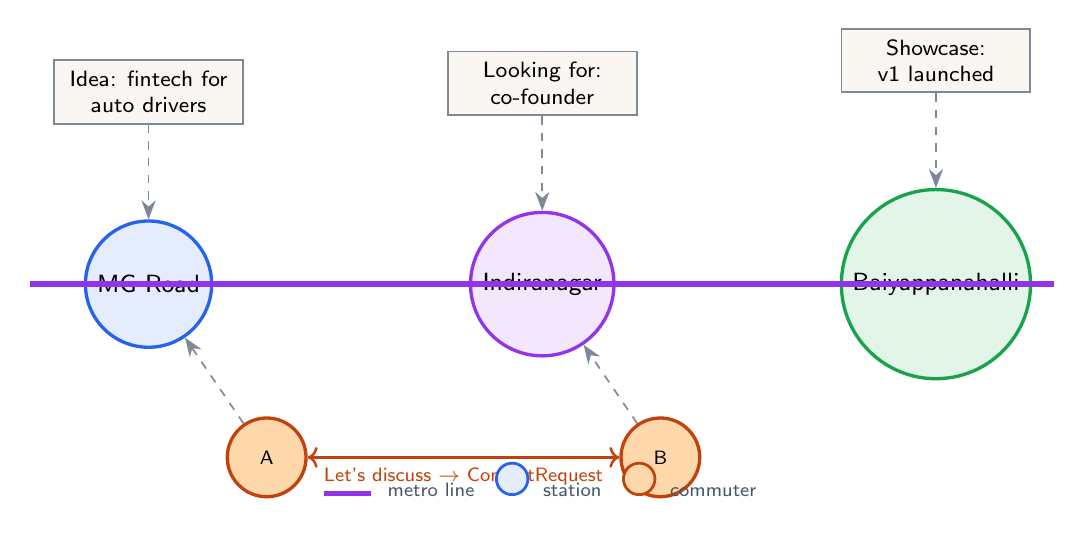
\begin{tikzpicture}[node distance=10mm and 14mm]
  % Three station nodes along an imaginary line, each in a different metro colour
  \node[circle, draw=metroblue, line width=1.2pt, fill=metroblue!12,
        minimum size=14mm, font=\small\sffamily] (s1) at (-5,0) {MG Road};
  \node[circle, draw=metropurple, line width=1.2pt, fill=metropurple!12,
        minimum size=14mm, font=\small\sffamily] (s2) at (0,0) {Indiranagar};
  \node[circle, draw=metrogreen, line width=1.2pt, fill=metrogreen!12,
        minimum size=14mm, font=\small\sffamily] (s3) at (5,0) {Baiyappanahalli};

  % Line connecting them
  \draw[metropurple, line width=2pt] (-6.5,0) -- (6.5,0);

  % Idea posts anchored above each station
  \node[entity, above=12mm of s1, minimum width=24mm] (i1)
    {Idea: fintech for\\auto drivers};
  \node[entity, above=12mm of s2, minimum width=24mm] (i2)
    {Looking for:\\co-founder};
  \node[entity, above=12mm of s3, minimum width=24mm] (i3)
    {Showcase:\\v1 launched};

  \draw[dashedarrow] (i1) -- (s1);
  \draw[dashedarrow] (i2) -- (s2);
  \draw[dashedarrow] (i3) -- (s3);

  % Two commuter avatars below, connected by "Let's discuss"
  \node[circle, draw=terracotta, line width=1.2pt, fill=terracottatint,
        minimum size=10mm, font=\scriptsize\sffamily] (u1) at (-3.5,-2.2) {A};
  \node[circle, draw=terracotta, line width=1.2pt, fill=terracottatint,
        minimum size=10mm, font=\scriptsize\sffamily] (u2) at (1.5,-2.2) {B};

  % "Let's discuss" link
  \draw[flow, <->] (u1) -- node[below, font=\scriptsize\sffamily, color=terracotta] {Let's discuss $\to$ ContactRequest} (u2);

  % Tie commuters to their home stations
  \draw[dashedarrow] (u1) -- (s1);
  \draw[dashedarrow] (u2) -- (s2);

  % Legend (below the figure, centred on s2)
  \node[font=\scriptsize\sffamily, color=slate, anchor=north, align=center]
    at ([yshift=-12mm]s2.south) {
    \tikz\draw[metropurple, line width=2pt] (0,0) -- (6mm,0);~ metro line\quad
    \tikz\draw[draw=metroblue, fill=metroblue!12, line width=1pt] (0,0) circle (2mm);~ station\quad
    \tikz\draw[draw=terracotta, fill=terracottatint, line width=1pt] (0,0) circle (2mm);~ commuter
  };
\end{tikzpicture}
\caption{Idea Junction concept. Stations (coloured by metro line) sit along a
route. Each idea is anchored to a single station. Commuters associated with a
station see ideas there first. The "Let's discuss" action creates a
\texttt{ContactRequest} between two commuters, gated by mutual acceptance
before any contact information is exchanged.}
\label{fig:idea}
\end{figure}

\subsection{Why station-anchored entrepreneurship is novel}

Existing founder-matching platforms (Y Combinator Co-Founder Matching,
Wellfound, indiehackers) match on skill, interest, or geography at the city
level. None of them match on shared routine. Two people who both ride the
Purple Line in Bengaluru at 8:45 each morning have something the city-level
platforms do not capture: a recurring block of involuntary co-presence. That
block is long enough for a serious conversation, predictable enough to plan
around, and physically co-located, which removes the friction of scheduling a
video call. Idea Junction exploits exactly that.

The station anchor also does a second job: it filters the noise. A founder in
Bengaluru asking about cofounders sees ideas from other Bengaluru commuters
first, not a global feed of half-finished pitches. The station is a soft
reputation proxy too: someone who posts repeatedly from the same station is
probably a regular, which makes them easier to find at the platform if a
conversation goes well online.

\subsection{Data fields and lifecycle}

An Idea record carries the following fields:

\begin{itemize}[leftmargin=1.4em, itemsep=2pt, topsep=2pt]
  \item \texttt{id}, \texttt{authorId}, \texttt{stationCode}, \texttt{createdAt}
  \item \texttt{title}, \texttt{description}
  \item \texttt{category}: \texttt{idea} $\mid$ \texttt{feedback} $\mid$ \texttt{cofounder} $\mid$ \texttt{discussion} $\mid$ \texttt{showcase}
  \item \texttt{lookingFor}: \texttt{co-founder} $\mid$ \texttt{feedback} $\mid$ \texttt{discussion} $\mid$ \texttt{collaborator}
  \item \texttt{stage}: \texttt{just-an-idea} $\mid$ \texttt{validating} $\mid$ \texttt{building} $\mid$ \texttt{launched}
  \item \texttt{status}: \texttt{open} $\mid$ \texttt{closed}
\end{itemize}

\noindent
The lifecycle is straightforward. An idea is created in the \texttt{open}
status. The author can update the stage as the project progresses (from
\texttt{just-an-idea} to \texttt{validating} to \texttt{building} to
\texttt{launched}), and can close the idea when the search is complete. Other
users can filter the board by any combination of the categorical fields. The
"Let's discuss" button is the only state-changing action available to a
non-author; it creates a \texttt{ContactRequest} and otherwise leaves the idea
record untouched.

% ============================================================================
%  8. FRONTEND ARCHITECTURE
% ============================================================================

\section{Frontend architecture}

The frontend is a Next.js App Router application. Routes are organised in two
groups. Public routes (the landing page, the about page, the station
directory, the sitemap, the robots file) are statically rendered at build
time. They depend only on the static station module and on no user state, so
they ship as plain HTML and are served from Vercel's edge network.
Application routes (the dashboard, the feed, carpools, lost-and-found,
marketplace, Idea Junction, the profile, and the auth pages) are client
components. They read from the Zustand store on the client and never run on
the server.

\subsection{Rendering strategy}

The split is deliberate. Public pages benefit from server rendering because
they are crawlable, fast on first paint, and cacheable at the edge. The
application pages benefit from client rendering because all of their data is
in the browser, and server rendering them would only produce a shell that the
client then has to hydrate and replace. Mixing the two is what the App Router
is designed for, and we use it as intended: server components where they help,
client components where they are necessary.

\subsection{State management}

State management is Zustand. Components subscribe to slices of the store via
selectors, so a change to the feed slice does not re-render a component that
only reads the carpool slice. The store is created once at module scope and
imported where needed; there is no provider in the React tree, which keeps
the component hierarchy flat.

\subsection{Motion}

Animation is Framer Motion at level 1. We use it for hover transitions, dialog
open and close, tab switches, and small list-item entrances. There are no
parallax effects, no scroll-driven animations, and no page transitions that
would slow the user down. The intent is to make the app feel responsive
without making it feel decorative.

\subsection{Listing: a Zustand store slice}

To make the persistence pattern concrete, the listing below shows the
shape of the Idea Junction slice and its two actions. The full store has the
same structure for every feature.

\begin{lstlisting}[caption={Idea Junction slice of the Zustand store (excerpt).},
                  label={lst:store}]
type IdeaCategory = "idea" | "feedback" | "cofounder" | "discussion" | "showcase";
type IdeaStage    = "just-an-idea" | "validating" | "building" | "launched";
type LookingFor   = "co-founder" | "feedback" | "discussion" | "collaborator";

interface Idea {
  id: string;
  authorId: string;
  stationCode: string;
  title: string;
  description: string;
  category: IdeaCategory;
  lookingFor: LookingFor;
  stage: IdeaStage;
  status: "open" | "closed";
  createdAt: number;
}

interface IdeaSlice {
  ideas: Idea[];
  addIdea: (input: Omit<Idea, "id" | "createdAt" | "status">) => void;
  closeIdea: (id: string) => void;
}

// Inside the create() call:
addIdea: (input) => set((state) => ({
  ideas: [
    { ...input, id: crypto.randomUUID(), createdAt: Date.now(), status: "open" },
    ...state.ideas,
  ],
})),
closeIdea: (id) => set((state) => ({
  ideas: state.ideas.map((i) => i.id === id ? { ...i, status: "closed" } : i),
})),
\end{lstlisting}

The persist middleware wraps the entire store. On every \texttt{set} call, the
new state is serialised and written to \texttt{localStorage} under
\texttt{metromitra-store}. The middleware also handles rehydration on boot,
so the listing above is the entire persistence story for ideas; nothing else
is required.

% ============================================================================
%  9. DEPLOYMENT AND CI/CD
% ============================================================================

\section{Deployment and CI/CD}

Deployment is to Vercel. There is no database to provision, no migration to
run, and no environment variable beyond the Vercel project configuration. The
build is \texttt{next build}, the output is static and edge-rendered pages,
and Vercel serves them. Figure~\ref{fig:deploy} shows the topology.

\begin{figure}[ht]
\centering
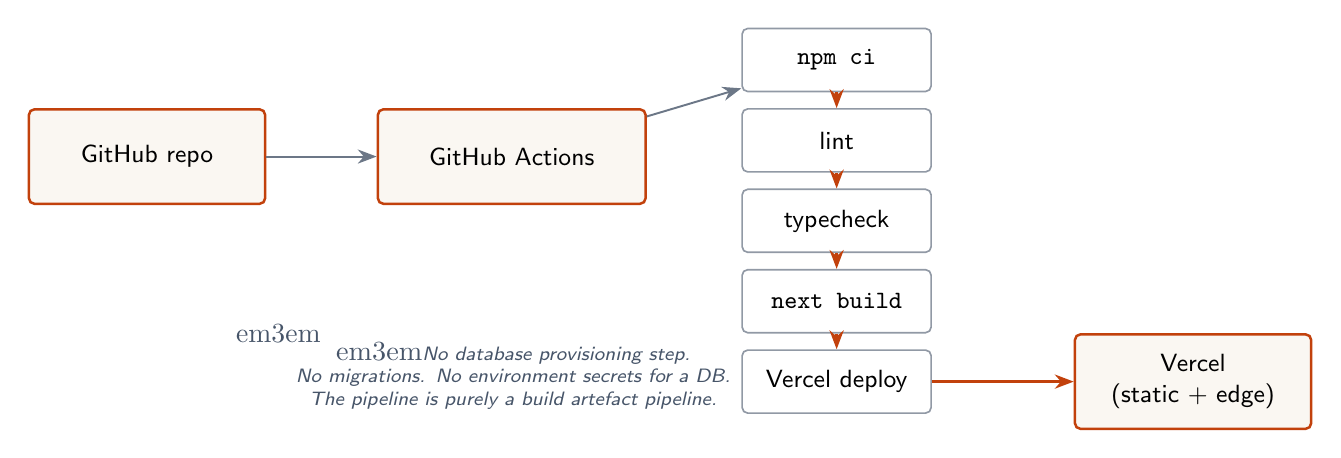
\begin{tikzpicture}[node distance=10mm and 14mm]
  % GitHub
  \node[block, minimum width=30mm, minimum height=12mm] (gh) {GitHub repo};
  % GitHub Actions
  \node[block, right=of gh, minimum width=34mm, minimum height=12mm] (gha) {GitHub Actions};
  % Pipeline inside GHA (a small column)
  \node[box, above right=2mm and 12mm of gha, minimum width=24mm] (ci) {\texttt{npm ci}};
  \node[box, below=2mm of ci, minimum width=24mm] (lint) {lint};
  \node[box, below=2mm of lint, minimum width=24mm] (tsc) {typecheck};
  \node[box, below=2mm of tsc, minimum width=24mm] (build) {\texttt{next build}};
  \node[box, below=2mm of build, minimum width=24mm] (deploy) {Vercel deploy};

  \draw[flow] (ci) -- (lint);
  \draw[flow] (lint) -- (tsc);
  \draw[flow] (tsc) -- (build);
  \draw[flow] (build) -- (deploy);

  % Vercel
  \node[block, right=18mm of deploy, minimum width=30mm, minimum height=12mm] (vercel) {Vercel\\(static + edge)};

  \draw[arrow] (gh) -- (gha);
  \draw[arrow] (gha) -- (ci);
  \draw[flow] (deploy) -- (vercel);

  % Explicit "no DB" annotation
  \node[font=\scriptsize\sffamily\itshape, color=slate, below=14mm of gha, align=center, text width=70mm]
    {No database provisioning step.\\No migrations. No environment secrets for a DB.\\
     The pipeline is purely a build artefact pipeline.};
\end{tikzpicture}
\caption{Deployment topology. A push or pull request to the GitHub repository
triggers GitHub Actions, which runs \texttt{npm ci}, lint, typecheck, and
\texttt{next build}. On push to \texttt{main} the workflow deploys the build
to Vercel. There is no database step because there is no database.}
\label{fig:deploy}
\end{figure}

\subsection{The pipeline}

The CI workflow runs on every push and every pull request. It does four
things: install dependencies with \texttt{npm ci}, run the linter, run the
TypeScript compiler in no-emit mode, and run \texttt{next build}. The build
step is the most important because it confirms that the production bundle
compiles. If any step fails the workflow stops and the pull request is
blocked.

A separate deploy job runs only on push to \texttt{main}. It uses the Vercel
CLI to build and deploy the production bundle. Concurrency cancellation is
enabled so that a new push to \texttt{main} cancels any in-flight deploy,
which keeps the deploy pipeline from queuing stale builds. The deploy job
does not run migrations, does not seed a database, and does not set
environment variables for a database connection, because none of those things
exist in this architecture.

\subsection{Why this works}

The pipeline is short because the architecture is short. The entire
application is a static asset bundle plus a small amount of edge rendering.
Vercel handles the asset distribution, the HTTPS termination, and the
compression. GitHub Actions handles the quality gate. There is no operational
surface beyond those two services, which is exactly the point of the
no-backend decision: the demo has nothing to operate.

% ============================================================================
%  10. SECURITY AND PRIVACY
% ============================================================================

\section{Security and privacy}
\label{sec:security}

The security posture of this release is honest about its limits. The
following are true and worth stating plainly.

\texttt{localStorage} is not secure. Any script running on the page can read
it, and any user with devtools access can read and modify it. The store
contains user records (with hashed but not salted passwords), posts, ideas,
carpools, contact requests, and the current session identifier. A reviewer
who opens devtools sees all of it.

The demo hash is not a cryptographic password hash. It is a one-way function
sufficient to keep plaintext passwords out of \texttt{localStorage}, and
nothing more. It is not salted per user, not slow, and not resistant to a
determined attacker who has the hash. We use it because the alternative in a
no-backend demo is plaintext, which is worse.

There is no server to enforce authorization. A user who knows another user's
id can construct a store mutation that references it. The UI does not expose
these paths, but the store is a public object and we do not pretend
otherwise.

Contact information is gated behind mutual acceptance. A user's phone number
or email is stored on their User record but is only surfaced to another user
after that user has sent a ContactRequest and the recipient has accepted it.
This is a privacy pattern, not a security control: it stops casual browsing
of contact details, not a determined attacker with devtools open.

There are no real payments in the app. The marketplace is a listing board;
any exchange of money happens outside the app. We do not store payment
instruments and we do not process transactions.

\subsection{What a production version would need}

A production MetroMitra would require a real backend. Specifically: a
server-side password hash (scrypt or argon2, salted per user), a database
with proper schema and migrations (Postgres or a managed equivalent), an
authentication system that issues short-lived tokens and validates them on
the server, authorization checks on every mutation, rate limiting on
write endpoints, input validation on the server (not only on the client),
audit logging for sensitive actions, and a privacy policy covering the
contact details users choose to share. The migration path from the current
architecture is not throwaway work: the Zustand store shape maps cleanly to
a set of API resources, the TypeScript types map to a schema, and the
component layer is largely unchanged because it already goes through a
selector-and-action indirection rather than calling fetch directly.

% ============================================================================
%  11. ACCESSIBILITY AND PERFORMANCE
% ============================================================================

\section{Accessibility and performance}

Accessibility is treated as a baseline, not a feature. Semantic HTML is used
throughout: headings are heading elements, lists are list elements, dialogs
use the appropriate ARIA roles via shadcn/ui primitives. Interactive elements
have visible focus styles. Colour contrast on the terracotta accent against
the warm off-white canvas meets WCAG AA for text. The metro-line colours used
in Idea Junction badges are never the sole carrier of information; each badge
also carries a text label, so a colour-blind user sees the category name.

Keyboard navigation works on every interactive surface. Dialogs trap focus
while open and restore it on close. Forms have associated label elements and
submit on enter. There are no custom focus traps implemented by hand; we rely
on the primitives from shadcn/ui, which are tested.

Performance is bounded by the no-backend decision. There is no network
waterfall on the client because there is no network. The initial bundle
includes the static station dataset, which is small (thirty-nine records, a
few kilobytes gzipped). The store rehydrates synchronously from
\texttt{localStorage} on boot, so there is no loading state for return
visits. The largest cost on first paint is the JavaScript bundle itself,
which is dominated by the React and Next.js runtimes; the application code is
a small fraction of the total. We do not pursue aggressive code splitting in
this release because the app is small enough that the trade-off is not worth
the complexity.

% ============================================================================
%  12. LIMITATIONS AND FUTURE WORK
% ============================================================================

\section{Limitations and future work}
\label{sec:limitations}

The limitations of the no-backend architecture are the limitations of any
single-browser application.

Data is ephemeral per browser. A user who posts an idea on their laptop will
not see it on their phone. Two users on two devices cannot see each other's
posts at all. The demo is single-player in the strict sense: every action
the reviewer takes is visible only to them.

There is no backup. If a user clears their browser storage, their data is
gone. There is no server holding a copy. This is acceptable for a
functionality demo and unacceptable for a product with real users.

The store will eventually get slow. Zustand is fast for the dataset sizes we
expect in a demo (hundreds of records, not millions), but a sufficiently
large \texttt{localStorage} payload will slow down both writes (because the
persist middleware serialises the entire tree on every change) and boots
(because rehydration parses the entire tree). For a real product this would
push us toward normalised state, selective persistence, or a backend.

\subsection{Migration path}

The migration to a real backend is well-defined. The Zustand store shape is
already a sensible API shape: each slice corresponds to a resource, each
action corresponds to a POST or PATCH. The TypeScript types are reusable as
the basis for a schema (Prisma, Drizzle, or a hand-written SQL schema). The
React component layer is the part that changes least, because it already goes
through the store rather than calling fetch directly. The work is in the
middle: replacing store actions with API calls, adding a real auth layer,
and adding the operational tooling (migrations, monitoring, backups) that a
real service requires.

\subsection{Idea Junction enrichment}

Idea Junction has clear room to grow. The current matching is implicit: a
user browses by station and category. A richer version would compute an
affinity score between a user and an idea based on shared stations, shared
ride times, and complementary skills (if the user profile carried skills).
Mentorship is a natural extension: a user who has launched a project could
opt in to mentor someone who is at the \texttt{just-an-idea} stage on the
same line. Pitch events are another: a station-anchored monthly virtual
pitch where the top three ideas posted that month get a five-minute slot
each. None of this is in the current release, but the data model is flexible
enough that none of it would require a rewrite.

% ============================================================================
%  13. CONCLUSION
% ============================================================================

\section{Conclusion}

MetroMitra v2 is a no-backend client-side application built to explore a
product concept, not to operate a service. Removing the server, the database,
and the API layer collapses the operational surface to a single static
bundle on Vercel, and collapses the developer setup to \texttt{npm install}
and \texttt{npm run dev}. The trade-off is that the app is single-browser
and demo-grade, and we are explicit about that throughout this document.

The Idea Junction feature is the reason the product is worth exploring. By
anchoring entrepreneurial ideas to metro stations, it ties founder search to
shared routine rather than shared geography, and it converts commute time
into a venue for serendipity. The data model, the store shape, and the
component architecture are all designed to make that feature first-class
without making the rest of the app feel secondary.

The path from here to a production product is clear. The local store maps to
a set of API resources. The TypeScript types map to a schema. The component
layer survives the migration largely intact. What we have built is a
faithful prototype of the product we would build for real, with the
engineering decisions documented honestly enough that the next stage of work
can start from this document rather than from the code.

\end{document}
